% Compilation : pdflatex Introduction_mecanique_des_fluides.tex (deux fois).
% Document autonome : texte, formules et figures TikZ modifiables.
% Les reperes Source renvoient aux pages du manuscrit.
\documentclass[11pt,a4paper]{article}
\usepackage[utf8]{inputenc}
\usepackage[T1]{fontenc}
\usepackage[provide=*,french]{babel}
\usepackage[scaled=.95]{helvet}
\renewcommand{\familydefault}{\sfdefault}
\usepackage{amsmath,amssymb,esint,array,tabularx}
\usepackage{geometry}
\geometry{left=15mm,right=15mm,top=18mm,bottom=18mm,headheight=14pt,headsep=6mm}
\usepackage{fancyhdr,lastpage,tikz}
\usetikzlibrary{arrows.meta,calc,decorations.pathreplacing,decorations.markings,patterns}
\usepackage[most]{tcolorbox}
\usepackage{enumitem,titlesec,needspace,hyperref}
\hypersetup{hidelinks,pdftitle={Introduction à la mécanique des fluides},pdfsubject={Cours de physique}}
\pagestyle{fancy}\fancyhf{}
\fancyhead[L]{\small Physique F1 - Introduction à la mécanique des fluides - inspiré par le cours de Mme Mesnil}
\fancyhead[R]{\small\thepage/\pageref{LastPage}}
\fancyfoot[R]{\small PC-PC*}
\renewcommand{\headrulewidth}{0pt}
\setlength{\parindent}{0pt}\setlength{\parskip}{5pt}
\setlength{\abovedisplayskip}{7pt}\setlength{\belowdisplayskip}{7pt}
\setlist[itemize]{leftmargin=5mm,itemsep=3pt,topsep=3pt,label=\(\rightarrow\)}
\setlist[enumerate]{leftmargin=6mm,itemsep=3pt,topsep=3pt}
\renewcommand{\thesection}{\Roman{section}}
\renewcommand{\thesubsection}{\thesection.\arabic{subsection}}
\titleformat{\section}{\Large\bfseries}{\thesection.}{.4em}{}
\titleformat{\subsection}{\large\bfseries}{\thesubsection.}{.4em}{}[\titlerule]
\titleformat{\subsubsection}{\normalsize\bfseries}{\alph{subsubsection})}{.5em}{}
\titlespacing*{\section}{0pt}{11pt}{6pt}
\titlespacing*{\subsection}{0pt}{9pt}{5pt}
\titlespacing*{\subsubsection}{0pt}{8pt}{4pt}
\newtcolorbox{cadre}[1][]{enhanced,sharp corners,colback=white,colframe=black,boxrule=1.1pt,left=7pt,right=7pt,top=5pt,bottom=5pt,before skip=7pt,after skip=7pt,#1}
\newtcolorbox{exemple}[1][]{enhanced,sharp corners,colback=white,colframe=black,boxrule=.7pt,left=8pt,right=8pt,top=6pt,bottom=6pt,before skip=8pt,after skip=8pt,#1}
\tcbset{etoiles/.style={width=\dimexpr\linewidth-22mm\relax,overlay={\node[anchor=west,inner sep=0pt,font=\small] at ([xshift=2mm]frame.east) {\(#1\)};}}}
\newcommand{\dd}{\mathrm d}
\newcommand{\vv}{\vec v}
\newcommand{\grad}{\overrightarrow{\mathrm{grad}}}
\newcommand{\pd}[2]{\frac{\partial #1}{\partial #2}}
\newcommand{\ux}{\vec u_x}\newcommand{\uy}{\vec u_y}\newcommand{\uz}{\vec u_z}
\newcommand{\cste}{\mathrm{cste}}
\newcommand{\titr}[1]{\par\needspace{4\baselineskip}\textbf{\underline{#1}}\par}
\newcommand{\planpart}[2]{\par\vspace{5pt}{\bfseries #1. #2}\par}
\newcommand{\plansub}[2]{\hspace*{7mm}{\itshape #1 #2}\par}
\newcommand{\plansubsub}[1]{\hspace*{15mm}{\itshape #1}\par}
\tikzset{>=Stealth,every node/.style={font=\small},flow/.style={thick,->},edge/.style={thick}}
% Une normale utilise le repere tangent/normal fourni par TikZ.
\tikzset{normale/.style args={#1/#2}{postaction={decorate},decoration={markings,mark=at position #1 with{\draw[flow] (0,0)--(0,#2);}}}}
\newcommand{\repere}[1]{\draw[->] (0,0)--(.8,0);\draw[->] (0,0)--(0,.8);\draw[->] (0,0)--(-.45,-.5);\node[below right] at (.15,-.1){$#1$};}
\newcommand{\canal}[1]{\begin{tikzpicture}[scale=.8]
\draw[edge] (0,2.4)..controls (2,2.6) and (4,2.6)..(6,2.6);
\draw[edge] (0,-.6)..controls (1.5,1.1) and (3.8,1.7)..(6,1.9);
\ifnum#1<3 \foreach \x/\y/\dx/\dy in {1/1.9/1/.08,2.6/1.6/1/.12,1.4/1.05/.8/.32}{\draw[flow] (\x,\y)--+(\dx,\dy);}\fi
\ifnum#1=1 \foreach \x/\y in {1/1.9,2.6/1.6,1.4/1.05,4/2.15}{\node at (\x,\y){$\times$};}\node[below,align=center] at (2,-.65){Traceurs : bulles de gaz, colorant,\\bouchons de liège, etc.};\draw (6.5,.7) rectangle (7.3,1.3);\draw (6.5,.8)--(6.15,.6)--(6.15,1.4)--(6.5,1.2);\node[below] at (6.8,.5){Caméra};\fi
\ifnum#1=2 \draw (2.6,1.6) circle (.22);\node[above] at (2.6,1.8){$M$};\fi
\ifnum#1=3
\tikzset{traceur/.style={postaction={decorate},decoration={markings,mark=at position .3 with{\draw[flow] (-.2,0)--(.7,0);\node[transform shape=false] at (-.2,0){$\times$};\node[transform shape=false] at (.05,0){$+$};}}}}
\draw[densely dotted,traceur] (.6,.4)..controls (2,1.2) and (4,1.85)..(6,2.05);
\draw[densely dotted,traceur] (.6,1.3)..controls (2,1.65) and (4,2.1)..(6,2.28);
\draw[densely dotted,traceur] (.6,2)..controls (2,2.15) and (4,2.35)..(6,2.4);
\path[postaction={decorate},decoration={markings,mark=at position .75 with{\draw[flow] (-.2,0)--(.7,0);\node[transform shape=false] at (-.2,0){$\times$};\node[transform shape=false] at (.05,0){$+$};}}] (.6,2)..controls (2,2.15) and (4,2.35)..(6,2.4);
\node[right,align=left] at (6.3,2){$\times$ : traceur à $t$\\$+$ : traceur à $t+\dd t$};\fi
\end{tikzpicture}}
\newcommand{\manege}[1]{\begin{tikzpicture}[scale=.82]
\draw[edge] (0,0) circle (1.5);\draw[edge] (0,0) circle (.52);\ifnum#1=2 \node at (.55,-.85){Huile};\else\node at (0,-.9){Huile};\fi
\draw[->] (1.85,-.4) arc (-20:35:1);\node[right] at (2,.2){$\omega$};
\ifnum#1=0 \draw[->] (.72,-.2) arc (-20:45:.65);\fi
\ifnum#1=1 \node[font=\scriptsize] at (0,0){$\vv=\vec0$};\fi\ifnum#1=2 \node[font=\scriptsize] at (0,0){$\vv\ne\vec0$};\fi\ifnum#1>0\ifnum#1<3 \foreach \a in {0,70,150,240}{\draw[flow,rotate=\a] (1.5,0)--(1.5,1);}\fi\fi
\ifnum#1=2 \foreach \a in {0,70,150,240}{\draw[dashed,rotate=\a] (0,0)--(1.7,0);\foreach \r in {.75,1,1.25}{\draw[flow,rotate=\a] (\r,0)--+(0,{.8*(\r-.5)});}}\fi
\ifnum#1=3 \draw[<->] (40:.6)--(40:1.45) node[midway,above left]{$L$};\draw[->] (.7,-.2) arc (-20:45:.65);\node[right] at (.7,.3){$\omega$};\fi
\end{tikzpicture}}
\newcommand{\cuve}[1]{\begin{tikzpicture}[scale=.82]
\draw[edge] (-1.5,2.7)--(-1.5,0)--(1.5,0)--(1.5,2.7);
\ifnum#1=0 \draw (-1.5,1.7)--(1.5,1.7);\draw[<->] (1.8,0)--(1.8,1.7) node[midway,right]{$h$};\node[left] at (-.4,-.45){$\omega=0$};\else
\draw[domain=-1.5:1.5,smooth,variable=\x] plot ({\x},{1.1+.27*\x*\x});
\draw[->] (0,-.25)--(0,3) node[above]{$\Delta$};\draw[->] (0,0)--(2.4,0) node[right]{$R'$};\draw[->] (0,0)--(-.65,-.65);
\ifnum#1=1 \draw[<->] (1.8,0)--(1.8,1.7) node[midway,right]{$h$};\fi
\ifnum#1=2 \draw[<->] (3.4,0)--(3.4,1.7) node[midway,right]{$h_0$};\draw[flow] (-1,1.37)--(-1.432,.57) node[left]{$\grad P$};\draw[flow] (1,1.37)--(1.432,.57) node[right]{$\grad P$};\fi
\ifnum#1=3 \draw[dashed] (0,1.1)--(1.5,1.1);\draw[<->] (1.8,0)--(1.8,1.1) node[midway,right]{$h$};\draw (.9,.45) circle (.1);\draw[flow] (.9,.45)--(.45,1.5) node[above]{$\vec\Pi_A$};\fi
\fi
\node at (-.7,.55){$\mu$};\draw[<->] (0,-.4)--(1.5,-.4) node[midway,below]{$R$};
\end{tikzpicture}}
\newcommand{\surfacefluide}{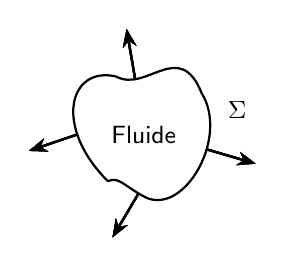
\begin{tikzpicture}[scale=.7]
\draw[edge,normale=.13/.65,normale=.38/.65,normale=.7/.65,normale=.92/.65] (0,0)..controls (-1,1) and (-.7,2.1)..(.15,1.9)..controls (.7,1.6) and (1.3,2.6)..(1.7,1.6)..controls (2.2,.8) and (1.4,-.6)..(.7,-.3)..controls (.3,-.1) and (.2,.1)..(0,0);
\node at (.65,.85){Fluide};\node[right] at (2,1.3){$\Sigma$};\end{tikzpicture}}
\newcommand{\cube}{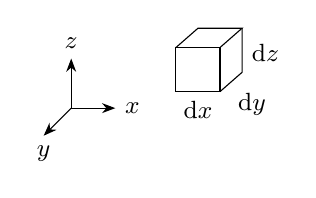
\begin{tikzpicture}[scale=.7]
\draw[->] (-.9,-.3)--(-.1,-.3) node[right]{$x$};\draw[->] (-.9,-.3)--(-.9,.6) node[above]{$z$};\draw[->] (-.9,-.3)--(-1.4,-.8) node[below]{$y$};
\draw (1,0) rectangle (1.8,.8);\draw (1,.8)--(1.4,1.15)--(2.2,1.15)--(1.8,.8);\draw (2.2,1.15)--(2.2,.35)--(1.8,0);\node[below] at (1.4,0){$\dd x$};\node[right] at (2.2,.7){$\dd z$};\node[below right] at (1.95,.15){$\dd y$};\end{tikzpicture}}
\begin{document}
{\fontsize{27}{31}\selectfont\bfseries Introduction à la mécanique des fluides\par}
\vspace{4mm}
\begingroup\setlength{\parskip}{3pt}
\planpart{I}{Description du mouvement d'un fluide}
\plansub{1)}{Qu'est-ce qu'un fluide ?}
\plansub{2)}{Qu'est-ce qu'un milieu continu}
\plansub{3)}{La particule fluide}
\plansub{4)}{Le champ des vitesses}
\plansubsub{a) Description eulérienne}
\plansubsub{b) Lignes de courant et tubes de courant}
\plansubsub{c) Écoulement stationnaire}
\planpart{II}{Actions mécaniques dans un fluide en mouvement}
\plansub{1)}{Forces agissant sur une particule fluide}
\plansub{2)}{Équivalent volumique des forces de pression}
\plansub{3)}{Approche expérimentale de la viscosité}
\plansub{4)}{Diffusion de la quantité de mouvement}
\plansub{5)}{Équivalent volumique de la force de viscosité de cisaillement}
\planpart{III}{Quelques caractéristiques d'un écoulement et conditions aux limites}
\plansub{1)}{Nombre de Reynolds}
\plansub{2)}{Écoulements laminaire et turbulent}
\plansub{3)}{Conditions aux limites}
\plansub{4)}{Modèle de l'écoulement parfait et notion de la couche limite}
\planpart{IV}{Traînée d'un solide dans un fluide}
\plansub{1)}{Position du problème}
\plansub{2)}{Expression de la force de traînée pour une sphère}
\planpart{V}{Statique des fluides en référentiel non galiléen}
\plansub{1)}{Liquide dans un récipient en translation dans un référentiel galiléen}
\plansub{2)}{Liquide dans une cuve en rotation uniforme autour d'un axe fixe dans un référentiel galiléen}
\endgroup
\par\vspace{8pt}
% Source : pages 1-3.
\begin{itemize}
\item Archimède.
\item Au XVII\textsuperscript{e} siècle, Pascal et Torricelli étudient la statique des fluides.
\item Au XVIII\textsuperscript{e} siècle, la dynamique des fluides se développe : Pitot étudie la vitesse d'écoulement ; Bernoulli met en équation la vitesse ; Euler et Lagrange mettent en équation la dynamique.
\item Au XIX\textsuperscript{e} siècle interviennent Navier, Poiseuille, Helmholtz, Mach et Reynolds.
\item En 1904, Prandtl est un pionnier de la couche limite.
\end{itemize}
\needspace{10\baselineskip}
\section{Description du mouvement d'un fluide}
\subsection{Qu'est-ce qu'un fluide ?}
\titr{Définitions}
\begin{enumerate}
\item Un fluide est un milieu qui peut s'écouler.
\item Un fluide est un corps qui prend la forme du récipient qui le contient.
\end{enumerate}
Un fluide est un liquide ou un gaz, mais il existe des différences entre les deux.
\begin{enumerate}
\item \textbf{Volume :} un gaz occupe tout le volume, contrairement à un liquide.
\item \textbf{Compressibilité :} un gaz est facile à comprimer ; un liquide est peu compressible.
\item \textbf{Dilatation :} lorsque $T$ augmente, un gaz se dilate davantage qu'un liquide, mais un liquide se dilate aussi.
\item \textbf{Ordres de grandeur à température et pression ambiantes :}
\end{enumerate}
\begin{center}\renewcommand{\arraystretch}{1.5}
\begin{tabular}{l|c|c}
& Liquide & Gaz\\\hline
Masse volumique $\mu$ & $10^3\ \mathrm{kg\,m^{-3}}$ & $1\ \mathrm{kg\,m^{-3}}$\\
Densité particulaire $n$ & $3\cdot10^{29}\ \mathrm{m^{-3}}$ & $3\cdot10^{26}\ \mathrm{m^{-3}}$
\end{tabular}\end{center}
\subsection{Qu'est-ce qu'un milieu continu}
On distingue trois échelles.
\titr{Échelle microscopique}
À cette échelle, on voit le déplacement des molécules et les quantités microscopiques. Le milieu est discontinu. Les distances caractéristiques sont :
\begin{itemize}
\item la taille d'une molécule ;
\item la distance intermoléculaire $d=\dfrac1{\sqrt[3]{n}}$ ;
\item le libre parcours moyen $\ell$, distance parcourue par une molécule entre deux chocs successifs.
\end{itemize}
Pour un liquide, $\ell\simeq d$. À température et pression ambiantes, le libre parcours moyen vaut $0{,}3\ \mathrm{nm}$ pour l'eau liquide et $70\ \mathrm{nm}$ pour l'air. Dans la haute atmosphère, il atteint plusieurs mètres.
% Source : pages 3-7.
\titr{Échelle macroscopique}
C'est l'échelle de l'expérimentateur. La distance caractéristique dépend de l'expérience. \begin{exemple}
Par exemple, pour l'écoulement dans un tuyau, la distance caractéristique est le diamètre du tuyau.
\end{exemple}
\titr{Échelle mésoscopique}
On note $\ell$ la distance caractéristique microscopique, $L$ la distance caractéristique macroscopique et $D$ la distance caractéristique mésoscopique, telle que
\[\ell\ll D\ll L.\]
\begin{cadre}
L'\textbf{approximation des milieux continus} est la possibilité de définir une échelle mésoscopique où l'on peut, en un point $M$, calculer des valeurs moyennes sur une très grande quantité d'entités microscopiques. Ces grandeurs physiques varient continûment à l'échelle macroscopique.
\end{cadre}
\subsection{La particule fluide}
Une particule fluide est un volume de fluide à l'échelle mésoscopique.
\[\text{Volume}=D^3,\qquad\text{noté }\dd^3\tau.\]
L'ordre de grandeur usuel de sa taille est $10\ \mu\mathrm m$, soit $3\times10^{10}$ molécules dans un liquide et $3\times10^7$ molécules dans un gaz.
Les moyennes sur la particule sont $T(M,t)$, $\mu(M,t)$ et $P(M,t)$ : on a un équilibre thermodynamique local.
On suppose que le nombre de molécules est quasi constant, car il est très grand : on fait l'hypothèse d'un système fermé.
\subsection{Le champ des vitesses}
\subsubsection{Description eulérienne}
\begin{center}\canal{0}\end{center}
\titr{Description lagrangienne}
On suit chaque particule fluide.
\[
\begin{pmatrix}X(t_0)\\Y(t_0)\\Z(t_0)\end{pmatrix}_{t=t_0}
\longrightarrow
\begin{pmatrix}X(t)\\Y(t)\\Z(t)\end{pmatrix}_{t},\qquad
\vec V(t)=\begin{pmatrix}V_x(t)=\dfrac{\dd X}{\dd t}\\[4pt]V_y(t)=\dfrac{\dd Y}{\dd t}\\[4pt]V_z(t)=\dfrac{\dd Z}{\dd t}\end{pmatrix}.
\]
Pour décrire l'écoulement, on étudie la \textbf{trajectoire} de la particule.
% Source : pages 6-9.
\titr{Expérimentalement}
\begin{center}\canal{1}\end{center}
\textbf{Avantage :} cette description facilite l'étude du mouvement des particules avec les lois de la dynamique.

\textbf{Inconvénient :} il est difficile d'écrire les conditions aux limites, aux bords de l'écoulement, sur les murs, etc.
\titr{Description eulérienne}
À chaque instant, on découpe le fluide en particules élémentaires centrées sur l'ensemble des points courants $M$. On définit le champ des vitesses $\vv(M,t)$ de la particule fluide en $M$. Les variables d'espace et de temps sont indépendantes.
\begin{center}\canal{2}\end{center}
\textbf{Avantage :} cette description facilite l'écriture des conditions aux limites.

\textbf{Inconvénient :} il est difficile d'appliquer directement les lois de la dynamique.
\subsubsection{Lignes de courant et tubes de courant}
\titr{Ligne de courant}
Une ligne de courant est une ligne de champ du champ des vitesses : en tout point de cette ligne, sa tangente est parallèle au champ des vitesses. On se place à $t$ fixé.
\begin{center}\canal{3}\end{center}
\titr{Équations des lignes de courant}
Dans la base cartésienne :
\[
\dd\vec M\in\mathrm{LdC}\ \Longleftrightarrow\ \dd\vec M\parallel\vv(P,t),\qquad
\begin{pmatrix}\dd x\\\dd y\\\dd z\end{pmatrix}\parallel
\begin{pmatrix}v_x(x,y,z,t)\\v_y(x,y,z,t)\\v_z(x,y,z,t)\end{pmatrix}.
\]
\[\frac{\dd x}{v_x(x,y,z,t)}=\frac{\dd y}{v_y(x,y,z,t)}=\frac{\dd z}{v_z(x,y,z,t)}.\]
% Source : pages 9-11.
Dans la base cylindrique :
\[\frac{\dd r}{v_r(r,\theta,z,t)}=\frac{r\,\dd\theta}{v_\theta(r,\theta,z,t)}=\frac{\dd z}{v_z(r,\theta,z,t)}.\]
Dans la base sphérique :
\[\frac{\dd r}{v_r(r,\theta,\varphi,t)}=\frac{r\,\dd\theta}{v_\theta(r,\theta,\varphi,t)}=\frac{r\sin\theta\,\dd\varphi}{v_\varphi(r,\theta,\varphi,t)}.\]
\begin{cadre}[etoiles={\mathord{\star}\,\mathord{\star}\,\mathord{\star}}]
En général, $\mathrm{LdC}\ne\text{trajectoire}$. Pour une ligne de courant, $t$ est fixé ; pour une trajectoire, le temps se déroule.
\end{cadre}
\titr{Tube de courant}
Le tube de courant d'un contour est l'ensemble des lignes de courant passant par ce contour.
\begin{center}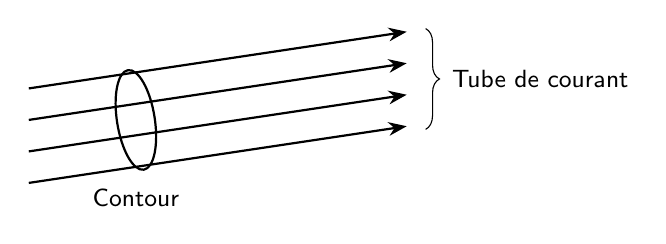
\begin{tikzpicture}[scale=.8]
\foreach \y in {-.75,-.25,.25,.75}{\draw[flow] (0,\y)--(6,\y+.9);}
\draw[thick,rotate around={9:(1.7,.25)}] (1.7,.25) ellipse (.3 and .8);
\node[below] at (1.7,-.7){Contour};\draw[decorate,decoration={brace,amplitude=5pt}] (6.3,1.7)--(6.3,.1) node[midway,right=6pt]{Tube de courant};
\end{tikzpicture}\end{center}
\titr{Filet de courant}
Un filet de courant est un tube de courant s'appuyant sur un contour élémentaire.
\titr{Remarque : lien mathématique entre les descriptions eulérienne et lagrangienne}
À partir de $\vv(M,t)$ :
\[\begin{aligned}
V_x(t)&=v_x\bigl(X(t),Y(t),Z(t),t\bigr),\\
V_y(t)&=v_y\bigl(X(t),Y(t),Z(t),t\bigr),\\
V_z(t)&=v_z\bigl(X(t),Y(t),Z(t),t\bigr).
\end{aligned}\]
Les majuscules correspondent à la description lagrangienne et les minuscules à la description eulérienne.
\subsubsection{Écoulement stationnaire}
Dans un référentiel donné, un écoulement est \textbf{stationnaire}, ou \textbf{permanent}, si les champs eulériens de vitesse, de masse volumique, de température, etc., sont tous indépendants du temps.
\[\vv(M)\qquad\text{ne dépend pas du temps.}\]
Il en résulte que :
\begin{enumerate}
\item les lignes de courant sont figées ;
\item les lignes de courant et les trajectoires sont superposées.
\end{enumerate}
% Source : pages 11-13.
\begin{exemple}
\titr{Exemples}
\textbf{1.} Le champ $\vv(M,t)=v\vec u(t)$ est uniforme.
\begin{center}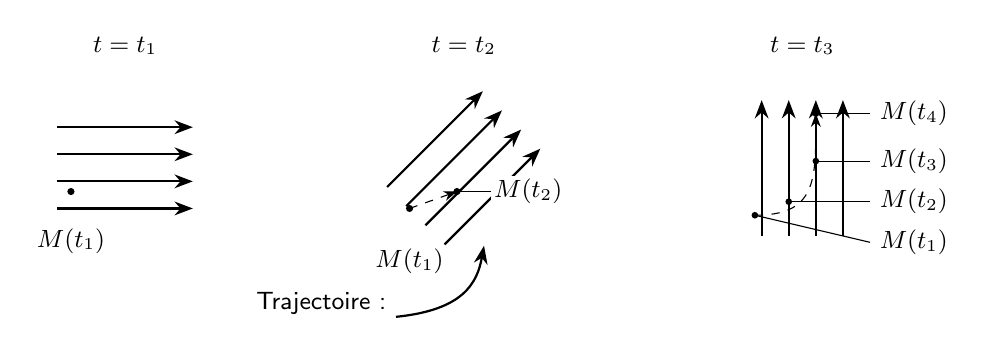
\begin{tikzpicture}[scale=.86]
\foreach \x/\a/\t in {0/0/1,5/45/2,10/90/3}{\begin{scope}[shift={(\x,0)}]
\node at (1,2.8){$t=t_{\t}$};\begin{scope}[rotate around={\a:(1,1)}]\foreach \y in {.4,.8,1.2,1.6}{\draw[flow] (0,\y)--(2,\y);}\end{scope}\end{scope}}
\fill (.2,.65) circle (1.5pt);\node[below] at (.2,.25){$M(t_1)$};
\draw[dashed,->] (5.2,.4)--(5.9,.65);\fill (5.2,.4) circle (1.5pt);\fill (5.9,.65) circle (1.5pt);
\node[below] at (5.2,-.05){$M(t_1)$};\node[right,fill=white,inner sep=1pt] at (6.4,.65){$M(t_2)$};\draw (5.9,.65)--(6.4,.65);
\draw[dashed,->] (10.3,.3)..controls (11.2,.3) and (11.2,.8)..(11.2,1.8);
\foreach \x/\y/\t/\labely in {10.3/.3/1/-.1,10.8/.5/2/.5,11.2/1.1/3/1.1,11.2/1.8/4/1.8}{\fill (\x,\y) circle (1.4pt);\draw[thin] (\x,\y)--(12,\labely);\node[right] at (12,\labely){$M(t_{\t})$};}
\node[left] at (5,-1){Trajectoire :};\draw[flow] (5,-1.2)..controls (6,-1.1) and (6.2,-.7)..(6.3,-.15);
\end{tikzpicture}\end{center}
\textbf{2.} Le champ $\vv(M,t)=v\vec u$ est uniforme et stationnaire.
\begin{center}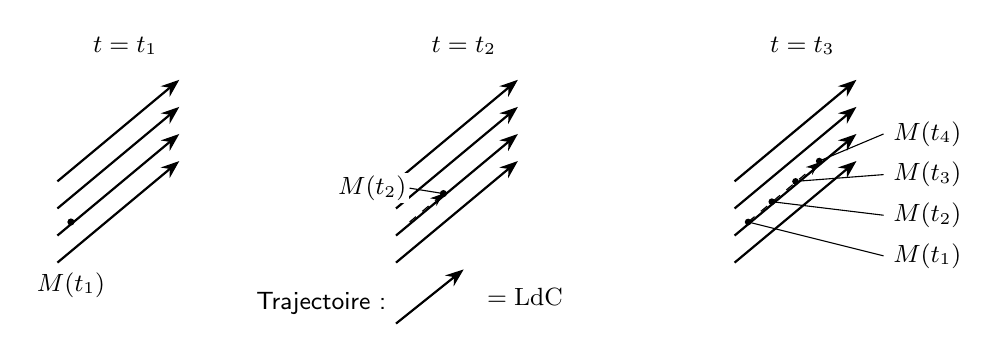
\begin{tikzpicture}[scale=.86]
\foreach \x/\t in {0/1,5/2,10/3}{\begin{scope}[shift={(\x,0)}]\node at (1,2.8){$t=t_{\t}$};\foreach \y in {-.4,0,.4,.8}{\draw[flow] (0,\y)--(1.8,\y+1.5);}\end{scope}}
\fill (.2,.2) circle (1.5pt);\node[below] at (.2,-.4){$M(t_1)$};
\draw[dashed,->] (5.2,.2)--(5.7,.62);\fill (5.7,.62) circle (1.5pt);\node[left,fill=white,inner sep=1pt] at (5.2,.7){$M(t_2)$};\draw (5.2,.7)--(5.7,.62);
\draw[dashed,->] (10.2,.2)--(11.25,1.08);
\foreach \x/\y/\t/\labely in {10.2/.2/1/-.3,10.55/.5/2/.3,10.9/.8/3/.9,11.25/1.1/4/1.5}{\fill (\x,\y) circle (1.4pt);\draw[thin] (\x,\y)--(12.2,\labely);\node[right] at (12.2,\labely){$M(t_{\t})$};}
\node[left] at (5,-1){Trajectoire :};\draw[flow] (5,-1.3)--(6,-.5);\node[right] at (6.2,-.9){$=\mathrm{LdC}$};
\end{tikzpicture}\end{center}
\end{exemple}
\textbf{Remarque :} le caractère stationnaire d'un écoulement dépend du référentiel d'étude.
\begin{exemple}
\titr{Exemple : un canard qui bouge}
Pour un observateur sur une berge, l'écoulement autour du canard est non stationnaire. Dans le référentiel lié au canard, l'écoulement est stationnaire.
\end{exemple}
\begin{exemple}
\titr{Exemple : le tourniquet hydraulique}
\begin{minipage}{.27\linewidth}\centering
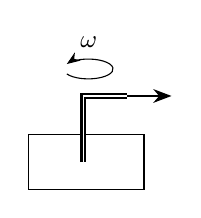
\begin{tikzpicture}[scale=.7]
\draw (0,0)--(0,1)--(2.1,1)--(2.1,0)--cycle;\draw[double,thick] (1,.5)--(1,1.7)--(1.8,1.7);\draw[flow] (1.8,1.7)--(2.6,1.7);\draw[->] (.7,2.1) arc (210:510:.45 and .18);\node[above] at (1.1,2.4){$\omega$};
\end{tikzpicture}
\end{minipage}\hfill\begin{minipage}{.7\linewidth}
Dans le référentiel $R$ du laboratoire, l'écoulement n'est pas stationnaire. Dans $R'$, lié au tourniquet, il est stationnaire.
\end{minipage}
\end{exemple}
\begin{exemple}
\titr{Exemple : le mascaret}
\begin{minipage}{.35\linewidth}\centering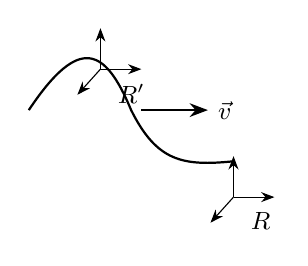
\begin{tikzpicture}[scale=.65]
\draw[thick] (-1,1)..controls (0,2.5) and (.5,2.2)..(1,1)..controls (1.5,0) and (2,-.1)..(3,0);
\begin{scope}[shift={(.4,1.8)}]\repere{R'}\end{scope}
\begin{scope}[shift={(3,-.7)}]\repere{R}\end{scope}
\draw[flow] (1.2,1)--(2.5,1) node[right]{$\vv$};
\end{tikzpicture}\end{minipage}\hfill\begin{minipage}{.62\linewidth}
Dans $R$, l'écoulement de la vague n'est pas stationnaire. Dans $R'$, lié au surfeur, il est stationnaire.
\end{minipage}
\end{exemple}
% Source : pages 13-15.
\section{Actions mécaniques dans un fluide en mouvement}
\subsection{Forces agissant sur une particule fluide}
Le système est une particule de fluide, assimilée à un solide déformable.
\begin{center}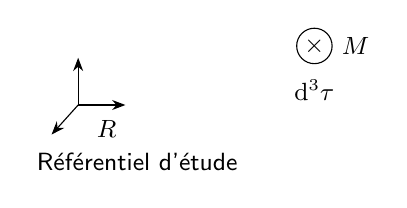
\begin{tikzpicture}[scale=.75]
\repere{R}\node[below] at (1,-.65){Référentiel d'étude};\draw (4,1) circle (.3);\node at (4,1){$\times$};\node[right] at (4.3,1){$M$};\node[below] at (4,.6){$\dd^3\tau$};
\end{tikzpicture}\end{center}
\titr{Forces extérieures $\vec F_{\mathrm{ext}}$}
\textbf{Forces à distance :}
\begin{cadre}\[\dd^3\vec f=\vec f_V\,\dd^3\tau.\]\end{cadre}
$\vec f_V$ est la densité volumique des forces à distance.

\begin{exemple}
\textbf{Exemple : le poids.}
\begin{cadre}[etoiles={\mathord{\star}\,\mathord{\star}\,\mathord{\star}\,\mathord{\star}}]\[\vec f_V=\mu(M,t)\vec g.\]\end{cadre}
$\mu$ est la masse volumique.
\end{exemple}
\begin{exemple}
\textbf{Exemple : la force de Lorentz.}
\[\vec f_V=\rho(M,t)\bigl[\vec E(M,t)+\vv(M,t)\wedge\vec B(M,t)\bigr].\]
$\rho$ est la densité volumique des charges.
\end{exemple}
\textbf{Forces de contact : $\dd^3\vec f$.} Les forces extérieures de contact en $\dd^2S$ se décomposent en
\[\dd^2\vec F=\dd^2\vec F_N+\dd^2\vec F_T,\qquad
\dd^2\vec F_N\parallel\vec n,\quad\dd^2\vec F_T\perp\vec n.\]
\begin{minipage}{.29\linewidth}\centering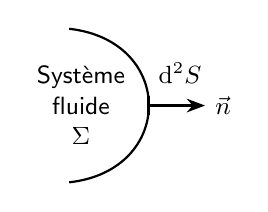
\begin{tikzpicture}[scale=.75]
\draw[thick] (0,-1.3)..controls (1.8,-1.1) and (1.8,1.1)..(0,1.3);
\draw[flow] (1.35,0)--(2.3,0) node[right]{$\vec n$};\draw[very thick] (1.34,-.16)--(1.34,.16);\node[above right] at (1.35,.2){$\dd^2S$};\node[align=center] at (.2,0){Système\\fluide\\$\Sigma$};
\end{tikzpicture}\end{minipage}\hfill\begin{minipage}{.67\linewidth}
La composante tangentielle est la force de viscosité. La composante normale est la force de pression :
\[\dd^2\vec F_N=-P(M,t)\,\dd^2\vec S.\]
Cf. partie suivante.
\end{minipage}
\titr{Forces intérieures $\vec F_{\mathrm{int}}$}
Les forces intermoléculaires sont dues aux chocs et aux interactions. Leur résultante est $\vec0$.
\titr{Forces d'inertie, si $R'$ est non galiléen}
\[\begin{aligned}
\dd^3\vec f_{ie}&=-\mu(M,t)\vec a_e(M,t)\,\dd^3\tau,\\
\dd^3\vec f_{ic}&=-\mu(M,t)\vec a_c(M,t)\,\dd^3\tau.
\end{aligned}\]
% Source : pages 14-17.
\subsection{Équivalent volumique des forces de pression}
Cf. sup.
\begin{cadre}[etoiles={\mathord{\star}\,\mathord{\star}\,\mathord{\star}\,\mathord{\star}\,\mathord{\star}}]\[\dd^3\vec f=-\grad P\,\dd^3\tau.\]\end{cadre}
\begin{minipage}{.32\linewidth}\centering\cube\end{minipage}\hfill\begin{minipage}{.65\linewidth}
\textbf{Attention :} cette expression s'applique uniquement à l'échelle mésoscopique.
\end{minipage}
\titr{Système macroscopique}
\begin{center}\surfacefluide\end{center}
\begin{cadre}\[
\vec F_{\text{résultante de pression}}
=\underbrace{\oiint_\Sigma -P(M,t)\,\dd^2\vec S}_{\text{intégrale de surface}}
=\underbrace{\iiint_V -\grad P\,\dd^3\tau}_{\text{intégrale sur tous les points}}.
\]\end{cadre}
\subsection{Approche expérimentale de la viscosité}
\begin{exemple}
\titr{Expérience 1 : le manège visqueux}
\begin{minipage}{.38\linewidth}\centering\manege{0}\end{minipage}\hfill\begin{minipage}{.58\linewidth}
La rotation du cylindre extérieur met l'huile en mouvement. L'huile entraîne la rotation du cylindre intérieur.

De même, lorsque la rotation du cylindre extérieur s'arrête brusquement, le cylindre intérieur s'immobilise.
\end{minipage}
\end{exemple}
\begin{exemple}
\titr{Expérience 2}
\begin{minipage}{.28\linewidth}\centering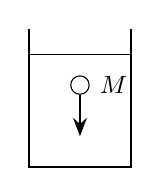
\begin{tikzpicture}[scale=.65]
\draw[thick] (0,2.7)--(0,0)--(2,0)--(2,2.7);\draw (0,2.2)--(2,2.2);\draw (1,1.6) circle (.18);\node[right] at (1.2,1.6){$M$};\draw[flow] (1,1.4)--(1,.6);
\end{tikzpicture}\end{minipage}\hfill\begin{minipage}{.68\linewidth}
Une bille $M$ chute dans un fluide visqueux. Elle atteint une vitesse limite.
\end{minipage}
\end{exemple}
% Source : pages 16-18.
\begin{exemple}
\titr{Expérience 3}
\begin{center}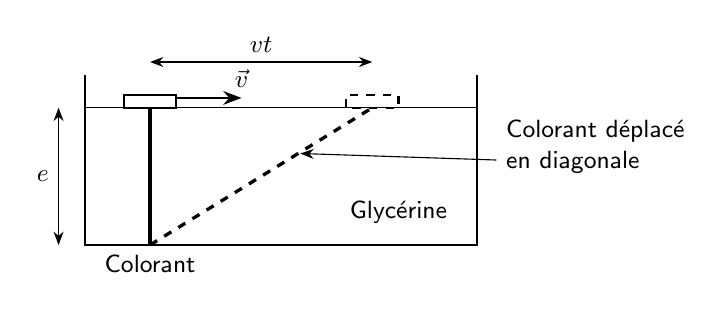
\begin{tikzpicture}[scale=.83]
\draw[thick] (0,2.6)--(0,0)--(6,0)--(6,2.6);\draw (0,2.1)--(6,2.1);
\draw[thick] (.6,2.1) rectangle (1.4,2.3);\draw[thick,dashed] (4,2.1) rectangle (4.8,2.3);
\draw[flow] (1.4,2.25)--(2.4,2.25) node[above]{$\vv$};
\draw[<->] (1,2.8)--(4.4,2.8) node[midway,above]{$vt$};
\draw[very thick] (1,0)--(1,2.1);\draw[very thick,dashed] (1,0)--(4.4,2.1);
\draw[<->] (-.4,0)--(-.4,2.1) node[midway,left]{$e$};
\node[below] at (1,0){Colorant};\node[right,align=left] at (6.3,1.5){Colorant déplacé\\en diagonale};\draw[->] (6.3,1.3)--(3.3,1.4);
\node at (4.8,.5){Glycérine};
\end{tikzpicture}\end{center}
La force tangentielle du palet sur le fluide déplace le fluide et le colorant. En bas, le fluide reste immobile à cause du frottement avec le sol.

On fait varier les paramètres suivants : la vitesse $v$, la hauteur de la colonne $e$ et la surface du palet $S$.
\begin{cadre}\[\vec F_{\mathrm{op}}=\eta\frac veS\ux.\]\end{cadre}
C'est une loi phénoménologique. Le coefficient $\eta$ dépend du liquide : c'est le \textbf{coefficient de viscosité dynamique}.
\[ [\eta]=\frac{[F][e]}{[v][S]}=\frac{MLT^{-2}\,L}{LT^{-1}\,L^2}.\]
\begin{cadre}\[ [\eta]=ML^{-1}T^{-1}.\]\end{cadre}
Unité : $\mathrm{kg\,s^{-1}\,m^{-1}}=\mathrm{Pl}$ (poiseuille).
\titr{Ordres de grandeur}
\begin{center}\renewcommand{\arraystretch}{1.3}\begin{tabular}{l|c}
Glycérine & $1\ \mathrm{Pl}$\\
Eau & $1\times10^{-3}\ \mathrm{Pl}$\\
Air & $1\times10^{-5}\ \mathrm{Pl}$
\end{tabular}\end{center}
\end{exemple}
\subsection{Diffusion de la quantité de mouvement}
\begin{center}
\begin{minipage}{.43\linewidth}\centering $t=0$\par\manege{1}\end{minipage}
\begin{minipage}{.43\linewidth}\centering $t=t_f$\par\manege{2}\end{minipage}
\end{center}
La viscosité entraîne une diffusion de la quantité de mouvement.
% Source : pages 19-21.
\needspace{7\baselineskip}
Il existe trois diffusions :
\begin{itemize}
\item la diffusion de particules, liée au gradient de concentration ;
\item la diffusion de chaleur, liée au gradient de température ;
\item la diffusion de quantité de mouvement.
\end{itemize}
Les deux premières seront étudiées en fin d'année. Les trois diffusions sont décrites par la même équation et ont le même moteur physique microscopique : l'agitation thermique.
\titr{Modélisation}
\begin{center}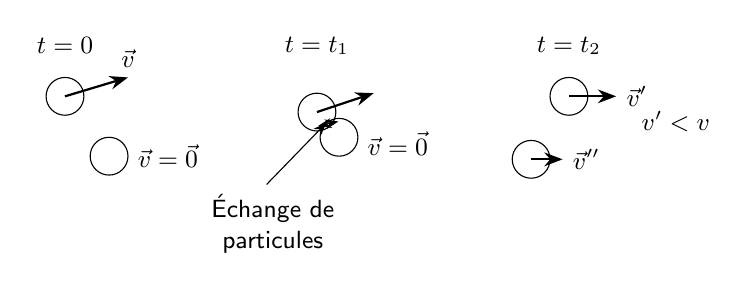
\begin{tikzpicture}[scale=.8]
\node at (0,1.4){$t=0$};\node at (4,1.4){$t=t_1$};\node at (8,1.4){$t=t_2$};
\draw (0,.6) circle (.3);\draw (.7,-.35) circle (.3);\draw[flow] (0,.6)--(1,.9) node[above]{$\vv$};\node[right] at (1,-.35){$\vv=\vec0$};
\draw (4,.35) circle (.3);\draw (4.35,-.05) circle (.3);\draw[flow] (4,.35)--(4.9,.65);\node[right] at (4.65,-.15){$\vv=\vec0$};\draw[<->] (4.02,.13)--(4.34,.2);\draw[->] (3.2,-.8)--(4.15,.18);\node[below,align=center] at (3.3,-.8){Échange de\\particules};
\draw (8,.6) circle (.3);\draw (7.4,-.4) circle (.3);\draw[flow] (8,.6)--(8.75,.6) node[right]{$\vv'$};\draw[flow] (7.4,-.4)--(7.9,-.4) node[right]{$\vv''$};\node[right] at (9,.2){$v'<v$};
\end{tikzpicture}\end{center}
\subsection{Équivalent volumique de la force de viscosité de cisaillement}
\begin{center}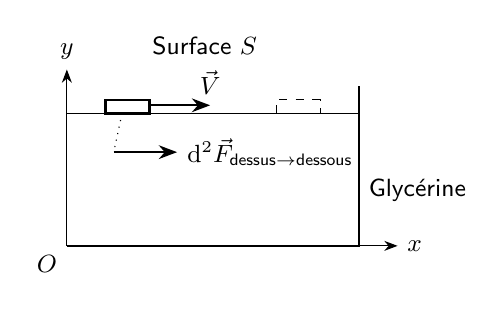
\begin{tikzpicture}[scale=.7]
\draw[->] (0,0)--(6,0) node[right]{$x$};\draw[->] (0,0)--(0,3.2) node[above]{$y$};\node[below left] at (0,0){$O$};\draw[thick] (0,0)--(5.3,0)--(5.3,2.9);\draw (0,2.4)--(5.3,2.4);
\draw[thick] (.7,2.4) rectangle (1.5,2.65);\draw[dashed] (3.8,2.4) rectangle (4.6,2.65);\draw[flow] (1.5,2.55)--(2.6,2.55) node[above]{$\vec V$};\node[above] at (2.5,3.3){Surface $S$};
\draw[dotted] (1,2.4)--(.85,1.7);\draw[flow] (.85,1.7)--(2,1.7) node[right]{$\dd^2\vec F_{\text{dessus}\to\text{dessous}}$};\node[right] at (5.3,1){Glycérine};
\end{tikzpicture}\end{center}
\[
\vec F_{\mathrm{op}}=\eta\frac VeS\ux,\qquad
\vv(M,t)=V\frac ye\ux
\quad\Longrightarrow\quad
\vec F_{\mathrm{op}}=\eta\pd{v_x}{y}S\ux=-\vec F_{\text{liquide}\to\text{palet}}.
\]
\textbf{Généralisation :} on admet que
\begin{cadre}[etoiles={\mathord{\star}\,\mathord{\star}\,\mathord{\star}\,\mathord{\star}}]\[
\dd^2\vec F_{\text{dessus}\to\text{dessous}}=\eta\,\dd^2S\,\ux\pd{v_x}{y}.
\]\end{cadre}
\begin{center}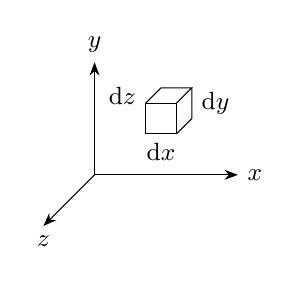
\begin{tikzpicture}[scale=.65]
\draw[->] (0,0)--(2.8,0) node[right]{$x$};\draw[->] (0,0)--(0,2.2) node[above]{$y$};\draw[->] (0,0)--(-1,-1) node[below]{$z$};
\draw (1,.8) rectangle (1.6,1.4);\draw (1,1.4)--(1.3,1.7)--(1.9,1.7)--(1.6,1.4);\draw (1.9,1.7)--(1.9,1.1)--(1.6,.8);\node[below] at (1.3,.8){$\dd x$};\node[right] at (1.9,1.4){$\dd y$};\node[left] at (1,1.55){$\dd z$};
\end{tikzpicture}\end{center}
% Source : pages 20-22. Corrections des étapes de calcul demandées par l’utilisateur.
\begin{align*}
\dd^3\vec F_{\mathrm{vis}}
&=\eta\,\dd x\,\dd z\left.\pd{v_x}{y}\right|_{y+\dd y}\ux
-\eta\,\dd x\,\dd z\left.\pd{v_x}{y}\right|_y\ux\\
&=\eta\,\dd x\,\dd z\,\ux\underbrace{\left[\left.\pd{v_x}{y}\right|_{y+\dd y}-\left.\pd{v_x}{y}\right|_y\right]}_{\simeq\,\dfrac{\partial^2v_x}{\partial y^2}\,\dd y=\dfrac{\dd^2v_x}{\dd y^2}\,\dd y}.
\end{align*}
\[\dd^3\vec F=\eta\,\dd x\,\dd y\,\dd z\,\frac{\partial^2v_x}{\partial y^2}\ux.\]
\begin{cadre}\[\dd^3\vec F=\eta\,\dd^3\tau\,\frac{\partial^2v_x}{\partial y^2}\ux.\]
\textit{Remarque sur cette formule :} elle correspond au cisaillement décrit par
\[\vv(M,t)=v_x(y,t)\ux.\]
L'écoulement se fait dans un sens et le cisaillement suivant une direction.
\end{cadre}
\titr{Généralisation à un écoulement quelconque}
Pour un écoulement incompressible et un fluide « newtonien » --- fluide pour lequel cette formule est vraie --- on a :
\begin{cadre}[etoiles={\mathord{\star}\,\mathord{\star}\,\mathord{\star}\,\mathord{\star}\,\mathord{\star}}]\[\dd^3\vec f_{\mathrm{vis}}=\eta\,\Delta\vv\,\dd^3\tau.\]\end{cadre}
$\Delta\vv$ est le laplacien de $\vv$ :
\[\begin{aligned}
\Delta v_x&=\frac{\partial^2v_x}{\partial x^2}+\frac{\partial^2v_x}{\partial y^2}+\frac{\partial^2v_x}{\partial z^2},\\[6pt]
\Delta v_y&=\frac{\partial^2v_y}{\partial x^2}+\frac{\partial^2v_y}{\partial y^2}+\frac{\partial^2v_y}{\partial z^2},\\[6pt]
\Delta v_z&=\frac{\partial^2v_z}{\partial x^2}+\frac{\partial^2v_z}{\partial y^2}+\frac{\partial^2v_z}{\partial z^2}.
\end{aligned}\]
% Source : pages 30-33.
\setcounter{section}{2}
\section{Quelques caractéristiques d'un écoulement et conditions aux limites}
\subsection{Nombre de Reynolds}
\begin{center}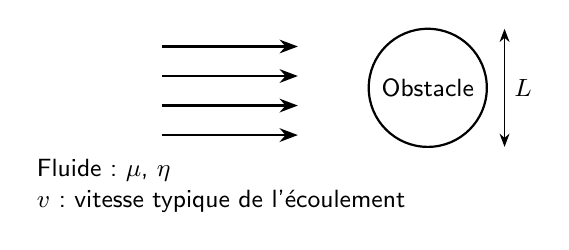
\begin{tikzpicture}[scale=.75]
\foreach \y in {0,.5,1,1.5}{\draw[flow] (0,\y)--(2.3,\y);}\node[below,align=left] at (1,-.25){Fluide : $\mu$, $\eta$\\$v$ : vitesse typique de l'écoulement};
\draw[thick] (4.5,.8) circle (1);\node at (4.5,.8){Obstacle};\draw[<->] (5.8,-.2)--(5.8,1.8) node[midway,right]{$L$};
\end{tikzpicture}\end{center}
On cherche à construire un nombre sans dimension pour décrire l'interaction fluide--obstacle.
\[[\mu]=\frac M{L^3},\qquad [\eta]=\frac M{LT},\qquad[v]=\frac LT,\qquad[L]=L.\]
\begin{cadre}\[R_e=\frac{\mu vL}{\eta},\qquad[R_e]=1.\]\end{cadre}
Le nombre de Reynolds est un nombre sans dimension caractérisant le mouvement du fluide, de masse volumique $\mu$, de vitesse typique $v$ et de viscosité $\eta$, autour d'un obstacle ou dans une conduite de dimension $L$.
\titr{Ordres de grandeur}
\begin{exemple}
\textbf{1. Une voiture dans l'air.}
\begin{center}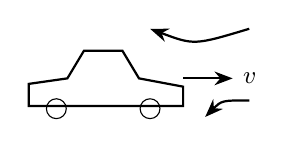
\begin{tikzpicture}[scale=.7]
\draw[thick] (0,0)--(0,.4)--(.7,.5)--(1,1)--(1.7,1)--(2,.5)--(2.8,.35)--(2.8,0)--cycle;\draw (.5,-.05) circle (.18);\draw (2.2,-.05) circle (.18);\draw[flow] (2.8,.5)--(3.7,.5) node[right]{$v$};\draw[flow] (4,1.4)..controls (3,1.1)..(2.2,1.4);\draw[flow] (4,.1)..controls (3.5,.1)..(3.2,-.2);
\end{tikzpicture}\end{center}
\[R_e=\frac{\mu_{\mathrm{air}}v_{\mathrm{voiture}}L}{\eta_{\mathrm{air}}},\qquad
L=2\ \mathrm m,\qquad v=v_{\mathrm{voiture}}=100\ \mathrm{km/h},\qquad R_e=10^6.\]
\end{exemple}
\begin{exemple}
\textbf{2. Le manège visqueux.}\par
\begin{minipage}{.39\linewidth}\centering\manege{3}\end{minipage}\hfill\begin{minipage}{.58\linewidth}
\[R_e=\frac{\mu_{\mathrm{huile}}vL}{\eta_{\mathrm{fluide}}}.\]
\[v\simeq20\ \mathrm{cm/s},\quad\eta_{\mathrm{huile}}=10^{-1}\ \mathrm{Pl},\]
\[L\simeq1\ \mathrm{cm},\qquad R_e\simeq1.\]
\end{minipage}
\end{exemple}
% Source : pages 33-35.
\titr{Interprétation}
\[R_e=\frac{\text{transport de quantité de mouvement par convection}}{\text{transport de quantité de mouvement par diffusion}}.\]
La convection correspond au mouvement global de matière. La démonstration sera donnée dans le cours de dynamique.
\begin{itemize}
\item Pour $R_e\gg1$, la convection domine.
\item Pour $R_e\ll1$, la diffusion domine.
\item Si $\eta\to0$, $R_e$ augmente : la convection domine.
\item Si $\eta\to\infty$, $R_e$ diminue : la diffusion domine.
\end{itemize}
Lorsque $R_e$ est petit, la viscosité joue un rôle important dans l'écoulement.
\subsection{Écoulements laminaire et turbulent}
Cf. poly.
\subsection{Conditions aux limites}
\begin{center}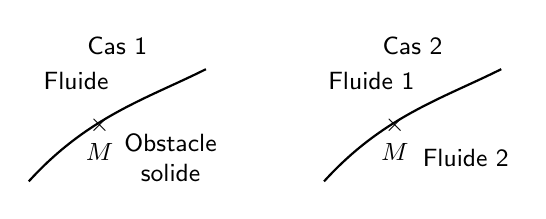
\begin{tikzpicture}[scale=.75]
\foreach \x/\titre in {0/Cas 1,5/Cas 2}{\begin{scope}[shift={(\x,0)}]\node at (1.5,2.3){\titre};\draw[thick] (0,0)..controls (1,1.1) and (2,1.4)..(3,1.9);\node at (1.2,.95){$\times$};\node[below] at (1.2,.8){$M$};\end{scope}}
\node at (.8,1.7){Fluide};\node[align=center] at (2.4,.4){Obstacle\\solide};\node at (5.8,1.7){Fluide 1};\node at (7.4,.4){Fluide 2};
\end{tikzpicture}\end{center}
En $M$, on distingue une condition limite cinématique, portant sur $\vv$, et une condition limite dynamique, portant sur les forces.
\titr{Cas 1}
\begin{center}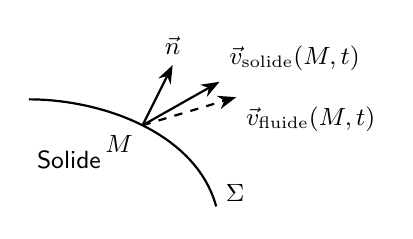
\begin{tikzpicture}[scale=.85]
\draw[thick] (-1.8,0)..controls (-.7,0) and (.7,-.5)..(1,-1.6);
% Point milieu de la cubique : tangente (3.15,-1.575), normale (1.575,3.15).
\coordinate (M) at (-.1,-.3875);\node[below left] at (M){$M$};\node at (-1.2,-.9){Solide};\node[right] at (1,-1.4){$\Sigma$};
\draw[flow] (M)--+(.45,.9) node[above]{$\vec n$};\draw[flow] (M)--+(1.15,.65);\node[above right] at (1.05,.28){$\vv_{\mathrm{solide}}(M,t)$};\draw[flow,dashed] (M)--+(1.4,.42);\node[below right] at (1.3,.03){$\vv_{\mathrm{fluide}}(M,t)$};
\end{tikzpicture}\end{center}
Un fluide réel accroche aux surfaces. La condition limite cinématique est
\[\vv_{\mathrm{fluide}}(M\in\Sigma,t)=\vv_{\mathrm{solide}}(M\in\Sigma,t).\]
On en déduit :
\[\vv_{\mathrm{fluide}}(M,t)\cdot\vec n=\vv_{\mathrm{solide}}(M,t)\cdot\vec n.\]
C'est la \textbf{condition d'impénétrabilité} du solide.
\par\needspace{5\baselineskip}
\[\vec v_{t,\mathrm{fluide}}(M,t)=\vec v_{t,\mathrm{solide}}(M,t).\]
C'est la \textbf{condition de non-glissement}. Les frottements traduisent les forces de viscosité.
% Source : pages 35-37.
\textbf{Cas d'un fluide non visqueux :} seule la condition d'impénétrabilité subsiste :
\[\vv_{\mathrm{fluide}}(M,t)\cdot\vec n=\vv_{\mathrm{solide}}(M,t)\cdot\vec n.\]
\titr{Cas 2}
\begin{center}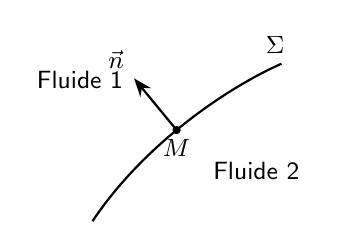
\begin{tikzpicture}[scale=.8]
\draw[thick] (-1.5,-1)..controls (-.7,.2) and (.6,1.1)..(1.5,1.5);
\path[postaction={decorate},decoration={markings,mark=at position .5 with{\fill (0,0) circle (1.5pt);\draw[flow] (0,0)--(0,.85) node[above left,transform shape=false]{$\vec n$};\node[below,transform shape=false] at (0,0){$M$};}}] (-1.5,-1)..controls (-.7,.2) and (.6,1.1)..(1.5,1.5);
\node at (-1.7,1.25){Fluide 1};\node at (1.1,-.2){Fluide 2};\node[above] at (1.4,1.5){$\Sigma$};
\end{tikzpicture}\end{center}
\[\vv_1(M\in\Sigma,t)=\vv_2(M,t).\]
\begin{itemize}
\item $\vv_1\cdot\vec n=\vv_2\cdot\vec n$ : c'est la condition d'impénétrabilité si les fluides ne se mélangent pas.
\item $\vec v_{t,1}=\vec v_{t,2}$ : c'est la condition de non-glissement, liée aux forces de viscosité.
\end{itemize}
\textbf{Cas non visqueux :} seule la condition d'impénétrabilité subsiste :
\[\vv_1\cdot\vec n=\vv_2\cdot\vec n.\]
\titr{Condition limite dynamique}
\begin{center}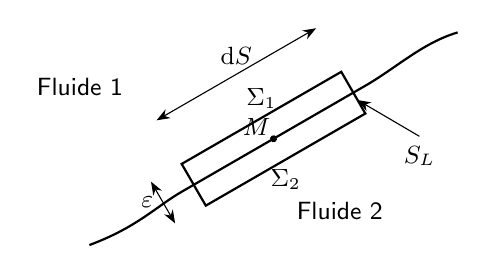
\begin{tikzpicture}[scale=.9]
\begin{scope}[rotate=30]
\draw[thick] (-3,0)..controls (-2.3,-.12) and (-1.9,0)..(-1.5,0)--(1.5,0)..controls (2,0) and (2.5,.12)..(3,0);
\draw[thick] (-1.3,-.34) rectangle (1.3,.34);
\fill (0,0) circle (1.4pt);\node[above left,inner sep=1pt] at (0,0){$M$};
\node[above] at (0,.34){$\Sigma_1$};\node[below] at (0,-.34){$\Sigma_2$};
\draw[<->] (-1.3,1.05)--(1.3,1.05) node[midway,above]{$\dd S$};
\draw[<->] (-1.8,-.34)--(-1.8,.34) node[midway,left]{$\varepsilon$};
\draw[->] (1.8,-1)--(1.3,-.12);\node[below] at (1.8,-1){$S_L$};
\node at (-2,2){Fluide 1};\node at (.3,-1.35){Fluide 2};
\end{scope}
\end{tikzpicture}\end{center}
On considère un parallélépipède fluide à cheval sur les deux milieux. Le théorème de la quantité de mouvement donne
\[\dd m\,\vec a=\vec f_{\mathrm{dist}}+\vec F_{\mathrm{contact}}+\vec f_{\mathrm{inertie}},\]
les forces de contact s'exerçant sur $\Sigma_1$, $\Sigma_2$ et $S_L$.
Pour $\varepsilon\to0$, on a $\dd m\to0$ et $\dd V\to0$. Alors
\[\vec0=\dd\vec F_{\Sigma_1}+\dd\vec F_{\Sigma_2}+\underbrace{\dd\vec F_{S_L}}_{\to\vec0}
=\dd\vec F_{\Sigma_1}+\dd\vec F_{\Sigma_2}.\]
% Source : pages 37-39.
On obtient, pour la composante normale et la composante tangentielle respectivement :
\[\left\{\begin{aligned}
&\forall M\in\Sigma,\quad P_1(M,t)=P_2(M,t),\\
&\dd^2\vec F_{\mathrm{tan},\,\text{dessus}\to\text{dessous}}
=-\dd^2\vec F_{\mathrm{tan},\,\text{dessous}\to\text{dessus}}.
\end{aligned}\right.\]
\begin{cadre}\[\left\{\begin{aligned}
&\forall M\in\Sigma,\quad P_1(M,t)=P_2(M,t),\\
&\dd^2\vec F_{\mathrm{vis},1,\,\text{dessus}\to\text{dessous}}
=\dd^2\vec F_{\mathrm{vis},2,\,\text{dessus}\to\text{dessous}}.
\end{aligned}\right.\]\end{cadre}
\titr{Récapitulation}
\begingroup\small\renewcommand{\arraystretch}{1.7}
\begin{tabularx}{\linewidth}{p{.18\linewidth}|X|X}
\textbf{Interface}&\textbf{Fluide non visqueux}&\textbf{Fluide visqueux}\\\hline
Solide/fluide&$\begin{aligned}\vv_{\mathrm{fluide}}(M,t)\cdot\vec n\\=\vv_{\mathrm{solide}}(M,t)\cdot\vec n\end{aligned}$&$\vv_{\mathrm{fluide}}(M,t)=\vv_{\mathrm{solide}}(M,t)$\\\hline
Fluide--fluide non miscibles&$\begin{aligned}\vv_{\mathrm{fluide}\,1}(M,t)\cdot\vec n\\=\vv_{\mathrm{fluide}\,2}(M,t)\cdot\vec n\end{aligned}$&$\begin{aligned}\vv_1(M,t)&=\vv_2(M,t),\\P_1(M,t)&=P_2(M,t),\\\dd^2\vec F_{\mathrm{vis}\,1}(M,t)&=\dd^2\vec F_{\mathrm{vis}\,2}(M,t).\end{aligned}$
\end{tabularx}\endgroup
\begin{exemple}
\titr{Exemple}
\begin{center}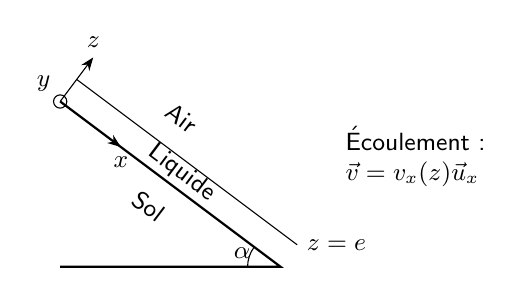
\begin{tikzpicture}[scale=.7]
\draw[thick] (0,3)--(4,0)--(0,0);\draw (0.3,3.4)--(4.3,.4);\draw[->] (0,3)--(1.1,2.175) node[below]{$x$};\draw[->] (0,3)--(.6,3.8) node[above]{$z$};\draw (0,3) circle (.12);\node[above left] at (0,3){$y$};\node[rotate=-37] at (2.2,1.7){Liquide};\node[rotate=-37] at (2.2,2.7){Air};\node[rotate=-37] at (1.6,1.1){Sol};\draw (3.4,0) arc (180:143:.6);\node at (3.3,.25){$\alpha$};\node[right] at (4.3,.4){$z=e$};\node[right,align=left] at (5,2){Écoulement :\\$\vv=v_x(z)\ux$};
\end{tikzpicture}\end{center}
\textbf{Conditions limites cinématiques}\par
\[z=0:\quad v_x(0)=0.\]
\[z=e:\quad\vec v_{x,\mathrm{liq}}(z=e)=\vec v_{x,\mathrm{air}}(z=e).\]
Cette dernière condition est inutile.
% Source : pages 39-41.
\par\medskip\textbf{Condition limite dynamique}\par
\begin{cadre}\[P(x,y,z=e)=P_0.\]\end{cadre}
\[\eta_{\mathrm{air}}\,\dd^2S\left.\pd{v_{x,\mathrm{air}}}{z}\right|_{z=e}\ux
=\eta_{\mathrm{liq}}\,\dd^2S\left.\pd{v_{x,\mathrm{liq}}}{z}\right|_{z=e}\ux.\]
Avec l'hypothèse $\eta_{\mathrm{air}}\simeq0$, on néglige la viscosité de l'air :
\[\left.\pd{v_{x,\mathrm{liq}}}{z}\right|_{z=e}=0.\]
\begin{center}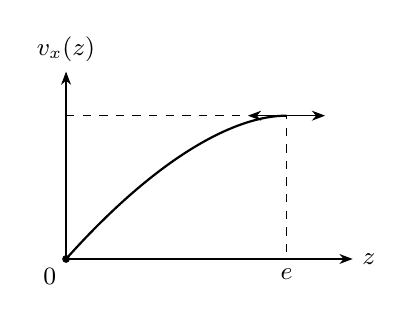
\begin{tikzpicture}[scale=.7]
\draw[->] (0,0)--(5.2,0) node[right]{$z$};\draw[->] (0,0)--(0,3.4) node[above]{$v_x(z)$};\node[below left] at (0,0){$0$};\draw[thick] (0,0)..controls (1.7,1.9) and (3.1,2.6)..(4,2.6);\fill (0,0) circle (2pt);\draw[dashed] (0,2.6)--(4,2.6)--(4,0);\node[below] at (4,0){$e$};\draw[<->] (3.3,2.6)--(4.7,2.6);
\end{tikzpicture}\end{center}
\end{exemple}
\subsection{Modèle de l'écoulement parfait et notion de la couche limite}
\textbf{Définition :} un écoulement parfait est un écoulement pour lequel tous les phénomènes diffusifs sont négligés, en particulier la diffusion de la quantité de mouvement, donc la viscosité.
\titr{Conséquences}
\begin{itemize}[beginpenalty=0,midpenalty=0,endpenalty=0]
\item La viscosité est négligée. Les seules forces de contact sont les forces de pression. \textbf{Attention :} il ne s'agit pas du champ de pression statique.
\item On néglige tous les phénomènes irréversibles. Toutes les particules subissent des transformations isentropiques : il n'y a ni échange de chaleur ni création d'entropie.
\end{itemize}
\par\penalty0
\[R_e=\frac{\text{transport de quantité de mouvement par convection}}{\text{transport de quantité de mouvement par diffusion}}.\]
On peut modéliser un écoulement par un écoulement parfait si $R_e\gg1$.
\begin{center}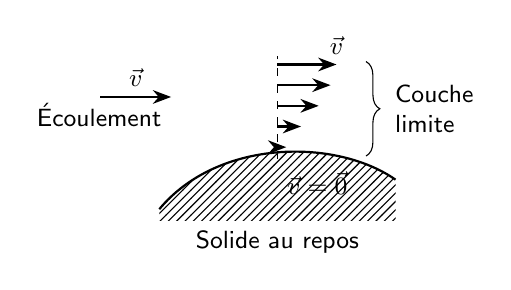
\begin{tikzpicture}[scale=.75]
\fill[pattern=north east lines] (-2,-.6)..controls (-1,.6) and (1,.6)..(2,-.1)--(2,-.8)--(-2,-.8)--cycle;
\draw[thick] (-2,-.6)..controls (-1,.6) and (1,.6)..(2,-.1);\node[below] at (0,-.8){Solide au repos};\draw[flow] (-3,1.3)--(-1.8,1.3) node[midway,above]{$\vv$};\node[left] at (-1.8,1){Écoulement};
\draw[dashed] (0,.25)--(0,2);\foreach \y/\v in {.45/.15,.8/.4,1.15/.7,1.5/.9,1.85/1}{\draw[flow] (0,\y)--(\v,\y);}\node[below right] at (0,.2){$\vv=\vec0$};\node[above] at (1,1.85){$\vv$};\draw[decorate,decoration={brace,amplitude=5pt}] (1.5,1.9)--(1.5,.3) node[midway,right=7pt,align=left]{Couche\\limite};
\end{tikzpicture}\end{center}
% Source : pages 41-43.
Les forces de viscosité ne sont pas négligeables très près de l'obstacle : c'est la couche limite. Elle assure la transition entre $\vv=\vec0$, due à l'accrochement au solide, et l'écoulement à la vitesse $\vv$.
Un écoulement réel à grand $R_e$ est assimilable à un écoulement parfait, sauf dans une couche de faible épaisseur autour des parois solides, la \textbf{couche limite}, dans laquelle les phénomènes de viscosité sont prédominants.
On note $\delta$ l'épaisseur de la couche limite et $L$ la distance caractéristique.
\begin{cadre}\[\delta=\frac L{\sqrt{R_e}}.\]\end{cadre}
\begin{exemple}
Autour d'une voiture à $90\ \mathrm{km/h}$, avec $L\sim2\ \mathrm m$, on a $R_e\sim10^6$ et $\delta\sim\mathrm{mm}$ : la couche limite est très fine.
\end{exemple}
\section{Traînée d'un solide dans un fluide}
\subsection{Position du problème}
\begin{center}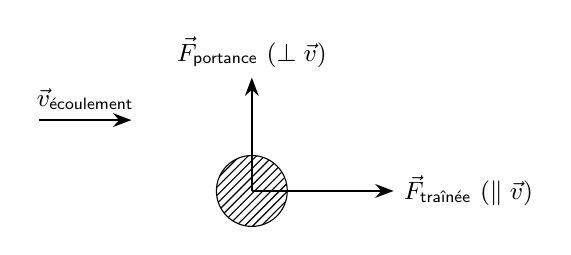
\begin{tikzpicture}[scale=.9]
\draw[flow] (-3,1)--(-1.7,1) node[midway,above]{$\vv_{\text{écoulement}}$};\draw[pattern=north east lines] (0,0) circle (.5);\draw[flow] (0,0)--(0,1.6) node[above]{$\vec F_{\text{portance}}\ (\perp\vv)$};\draw[flow] (0,0)--(2,0) node[right]{$\vec F_{\text{traînée}}\ (\parallel\vv)$};
\end{tikzpicture}\end{center}
\textbf{Attention :} $\vec F_{\text{portance}}$ n'est pas la poussée d'Archimède.
\subsection{Expression de la force de traînée pour une sphère}
\begin{center}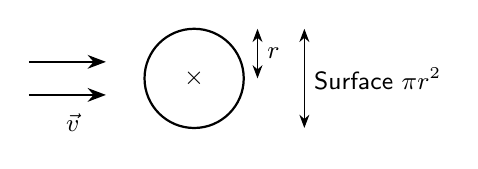
\begin{tikzpicture}[scale=.7]
\foreach \y in {-.3,.3}{\draw[flow] (-3,\y)--(-1.6,\y);}\node at (-2.2,-.8){$\vv$};\draw[thick] (0,0) circle (.9);\node at (0,0){$\times$};\draw[<->] (1.15,0)--(1.15,.9) node[midway,right]{$r$};\draw[<->] (2,-.9)--(2,.9) node[midway,right]{Surface $\pi r^2$};
\end{tikzpicture}\end{center}
\[R_e=\frac{\mu v(2r)}{\eta}.\]
\begin{cadre}\[C_x=\frac{f_{\text{traînée}}}{\tfrac12\mu_{\mathrm{fluide}}Sv^2}
=\frac{2f}{\mu_{\mathrm{fluide}}\pi r^2v^2}.\]\end{cadre}
Pour $R_e<1$ :
\begin{cadre}\[C_x=\frac{24}{R_e}.\]\end{cadre}
% Source : pages 43-45.
\[C_x=\frac{24}{R_e}=\frac{2f}{\mu_{\mathrm{fluide}}\pi r^2v^2}
=\frac{24}{2r}\frac{\eta_{\mathrm{fluide}}}{\mu_{\mathrm{fluide}}v}.\]
\[f=\frac{6\eta_{\mathrm{fluide}}}{\mu_{\mathrm{fluide}}rv}\,\mu_{\mathrm{fluide}}\pi r^2v^2,\qquad
f=6\eta_{\mathrm{fluide}}\pi rv.\]
Donc, pour $R_e<1$ :
\begin{cadre}[etoiles={\mathord{\star}\,\mathord{\star}\,\mathord{\star}\,\mathord{\star}}]\[\vec f_{\text{traînée}}=-6\pi\eta r\vv.\]\end{cadre}
Pour $2\times10^3<R_e<2\times10^5$, $C_x\simeq\cste=C$ et
\[f=\mu_{\mathrm{fluide}}\pi r^2\frac C2v^2.\]
\begin{cadre}[etoiles={\mathord{\star}\,\mathord{\star}\,\mathord{\star}\,\mathord{\star}\,\mathord{\star}}]\[\vec f_{\text{traînée}}=-\frac C2\mu_{\mathrm{fluide}}\pi r^2v\vv.\]\end{cadre}
\textbf{Autres zones :} il n'existe pas de formule générale.
\begin{exemple}
\titr{Exemple : chute d'une bille dans l'eau}
\[m=0{,}050\ \mathrm g,\qquad r=2{,}0\ \mathrm{mm}.\]
\textbf{Hypothèse :} $R_e<1$, à vérifier. Alors $\vec f=-6\pi\eta r\vv$.

On cherche la vitesse limite. Le théorème de la quantité de mouvement appliqué à la bille donne
\[m\vec a=m\vec g+\vec\Pi_A-6\pi\eta r\vv.\]
À la vitesse limite, $\vec a=\vec0$.
\begin{cadre}\[v=\frac{mg-\Pi_A}{6\pi\eta r}.\]\end{cadre}
Application numérique : $v=4\ \mathrm{m/s}$ et $R_e=2\times10^4$. \textbf{L'hypothèse est fausse.}

\textbf{Hypothèse :} $2\times10^3<R_e<2\times10^5$. De la même manière,
\[\vec0=m\vec g+\vec\Pi_A-\frac C2\mu_{\mathrm{fluide}}\pi r^2v\vv,\qquad
v=\sqrt{\frac{mg-\Pi_A}{\tfrac C2\mu_{\mathrm{fluide}}\pi r^2}}.\]
\[v\simeq0{,}2\ \mathrm{m\,s^{-1}},\qquad R_e\simeq7\times10^2.\]
L'hypothèse est fausse, mais elle n'est pas très éloignée du résultat. On est en régime intermédiaire ; la deuxième hypothèse est plus proche.
% Source : pages 45-46. Les pages 47 et 48 du fichier source sont vierges.
\end{exemple}
\par\penalty0
\par\textbf{\underline{Généralisation}}\par
Pour un objet quelconque dans l'écoulement :
\begin{cadre}\[R_e<1:\qquad\vec f=-\alpha\eta L\vv.\]\end{cadre}
La force est proportionnelle à $v$.\par\penalty0
\begin{cadre}\[R_e>10^3:\qquad\vec f=-\beta\mu_{\mathrm{fluide}}S_{\mathrm{app}}v\vv.\]\end{cadre}
La force est proportionnelle à $v^2$ et dépend de la surface apparente $S_{\mathrm{app}}$.\par\penalty0
\begin{exemple}
\titr{Expérience : deux cônes de papier}
Dans l'air, $\eta_{\mathrm{air}}=10^{-5}\ \mathrm{Pl}$ et $R_e\gg10^3$.
\[\vec f=-\beta\mu_{\mathrm{air}}S_{\mathrm{app}}v\vv,\qquad
v_{\mathrm{lim}}=\sqrt{\frac{mg}{\beta\mu S_{\mathrm{app}}}}.\]
Avec une surface apparente $S_{\mathrm{app}}$ plus grande, la vitesse limite $v_{\mathrm{lim}}$ est plus petite.
\end{exemple}
% Source : pages 22-25. Partie déplacée à la fin du cours à la demande de l’utilisateur.
\setcounter{section}{4}
\section{Statique des fluides en référentiel non galiléen}
\begin{center}\begin{tikzpicture}[scale=.8]
\repere{R_g}\begin{scope}[shift={(3,1)}]\repere{R'}\node[below] at (.4,-.7){Non galiléen};\end{scope}\draw (6,1.6) circle (.13);\node[above] at (6,1.8){$G$};\node[right] at (6.2,1.6){$\dd^3\tau$};
\end{tikzpicture}\end{center}
On applique le théorème de la quantité de mouvement à la particule :
\[\begin{aligned}
\dd^3M\,\vec a(G)={}&\underbrace{\vec f_V\,\dd^3\tau}_{\text{forces à distance}}
+\underbrace{\bigl(-\grad P+\eta\Delta\vv\bigr)\dd^3\tau}_{\text{pression et viscosité}}\\
&-\mu\vec a_e(G)\,\dd^3\tau-\mu\vec a_c(G)\,\dd^3\tau.
\end{aligned}\]
En statique, $\vv=\vec0$ et $\vec a=\vec0$. Ainsi,
\[\eta\Delta\vv=\vec0,\qquad\mu\vec a_c(G)\,\dd^3\tau=0,\]
\[\vec0=\vec f_V\,\dd^3\tau-\grad P\,\dd^3\tau-\mu\vec a_e(G)\,\dd^3\tau.\]
D'où :
\begin{cadre}\[\vec f_V=\grad P+\mu\vec a_e(G).\]\end{cadre}
\subsection{Liquide dans un récipient en translation dans un référentiel galiléen}
\begin{center}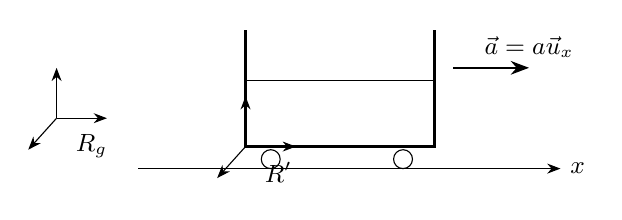
\begin{tikzpicture}[scale=.8]
\begin{scope}[shift={(-2,.8)}]\repere{R_g}\end{scope}
\draw[->] (-.7,0)--(6,0) node[right]{$x$};\draw[thick] (1,2.2)--(1,.35)--(4,.35)--(4,2.2);\draw (1,1.4)--(4,1.4);\draw (1.4,.15) circle (.15);\draw (3.5,.15) circle (.15);
\begin{scope}[shift={(1,.35)}]\repere{R'}\end{scope}\draw[flow] (4.3,1.6)--(5.5,1.6) node[above]{$\vec a=a\ux$};
\end{tikzpicture}\end{center}
Le référentiel $R'$, lié au chariot, est non galiléen. Il est en translation rectiligne uniformément accélérée par rapport à $R_g$.
On suppose que le liquide est au repos :
\[\vec f_V-\grad P-\mu\vec a_e=\vec0.\]
\begin{cadre}\[\mu\vec g=\grad P+\mu a\ux.\]\end{cadre}
% Source : pages 24-26.
Pour un liquide, $\mu$ est supposée constante :
\[-\mu g\uz=\grad P+\mu a\ux,\qquad\vec0=\grad\bigl(P+\mu ax+\mu gz\bigr).\]
Alors $P+\mu ax+\mu gz=\cste$, d'où
\begin{cadre}\[P=\cste-\mu ax-\mu gz.\]\end{cadre}
\titr{Autre méthode : méthode de sup}
\[\begin{aligned}
\pd P x&=-\mu a &&\Longrightarrow\quad P(x,y,z)=-\mu ax+f(y,z),\\
\pd P y&=0,\\
\pd P z&=-\mu g &&\Longrightarrow\quad P(x,y,z)=-\mu gz+f(x,y).
\end{aligned}\]
Donc $P=-\mu ax-\mu gz+\cste$.
\begin{center}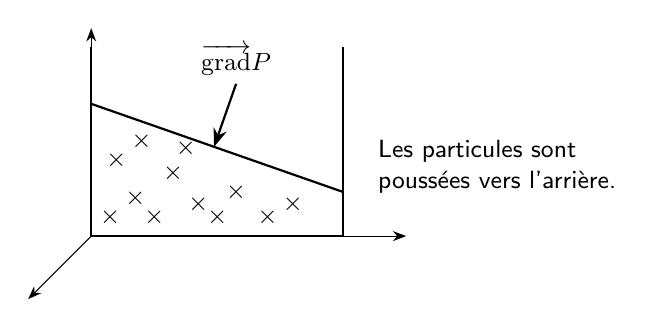
\begin{tikzpicture}[scale=.8]
\draw[->] (0,0)--(5,0);\draw[->] (0,0)--(0,3.3);\draw[->] (0,0)--(-1,-1);
\draw[thick] (0,3)--(0,0)--(4,0)--(4,3);\draw[thick] (0,2.1)--(4,.7);
\foreach \x/\y in {.3/.3,.7/.6,1/.3,1.3/1,1.7/.5,2/.3,2.3/.7,2.8/.3,3.2/.5,.4/1.2,.8/1.5,1.5/1.4}{\node at (\x,\y){$\times$};}
\draw[flow] (2.3,2.4175)--(1.95,1.4175);\node[above] at (2.3,2.4){$\grad P$};\node[right,align=left] at (4.4,1.1){Les particules sont\\poussées vers l'arrière.};
\end{tikzpicture}\end{center}
\titr{Surface libre}
Sur la surface, $P(M)=P_0$. Ainsi,
\[-\mu gz-\mu ax+\cste=P_0,\qquad z=-\frac agx+\cste'.\]
La surface libre est un plan.

\textbf{Remarque :} une surface isobare est perpendiculaire à $\grad P$.
\titr{Complément : poussée d'Archimède en référentiel non galiléen}
\begin{minipage}{.35\linewidth}\centering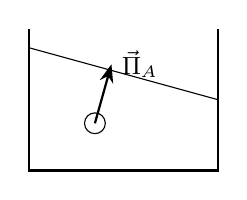
\begin{tikzpicture}[scale=.6]
\draw[thick] (0,3)--(0,0)--(4,0)--(4,3);\draw (0,2.6)--(4,1.5);\draw (1.4,1) circle (.22);\draw[flow] (1.4,1)--(1.75,2.25) node[right]{$\vec\Pi_A$};
\end{tikzpicture}\end{minipage}\hfill\begin{minipage}{.62\linewidth}
La direction de la poussée d'Archimède est liée aux forces d'inertie d'entraînement.
\end{minipage}
% Source : pages 26-28.
\titr{Complément : gaz parfait}
\[P=\frac{\mu RT}{M}.\]
On a toujours $\grad P=\mu\vec g-\mu a\ux$, soit
\[\left\{\begin{aligned}
\pd P x&=-\mu a=-\frac{PM}{RT}a,\\
\pd P y&=0,\\
\pd P z&=-\mu g=-\frac{PM}{RT}g.
\end{aligned}\right.\qquad P=P(x,z).\]
\[\begin{aligned}
\int\frac{\partial P}{P}&=-\frac{Ma}{RT}\,\partial x
&&\Longrightarrow\quad\ln P=-\frac{Ma}{RT}x+f(z),\\
\int\frac{\partial P}{P}&=-\frac{Mg}{RT}\,\partial z
&&\Longrightarrow\quad\ln P=-\frac{Mgz}{RT}+g(x).
\end{aligned}\]
\[\ln P=-\frac{Max}{RT}-\frac{Mgz}{RT}+k,\qquad
P(x,z)=k'\mathrm e^{-\frac{M}{RT}(ax+gz)}.\]
\subsection{Liquide dans une cuve en rotation uniforme autour d'un axe fixe dans un référentiel galiléen}
\begin{center}\cuve{0}\hspace{1cm}\cuve{1}\end{center}
Le référentiel $R_g$ est galiléen. Le référentiel $R'$, lié à la cuve en rotation uniforme autour de $\Delta$, est non galiléen.
Le référentiel d'étude est $R'$ ; le fluide y est au repos.
\[\begin{aligned}
\grad P&=\vec f_V-\mu\vec a_e\\
&=\mu\vec g+\mu\omega^2\overrightarrow{HM}\\
&=-\mu g\uz+\mu\omega^2r\vec u_r\\
&=\grad\left(-\mu gz+\tfrac12\mu\omega^2r^2\right).
\end{aligned}\]
\[\grad\left(P+\mu gz-\tfrac12\mu\omega^2r^2\right)=\vec0.\]
\begin{cadre}\[P(r,\theta,z)=K-\mu gz+\tfrac12\mu\omega^2r^2.\]\end{cadre}
% Source : pages 28-30.
\begin{center}\cuve{2}\end{center}
\titr{Surface libre}
Sur la surface libre, $P(M)=P_0$, donc
\[P_0=K-\mu gz+\tfrac12\mu\omega^2r^2.\]
Conditions initiales : $r=0$, $z=h$, $P=P_0$. Ainsi, $K=P_0+\mu gh$.
Donc
\[P_0=P_0+\mu gh-\mu gz+\tfrac12\mu\omega^2r^2.\]
\begin{cadre}\[z=h+\frac12\frac{\omega^2}{g}r^2.\]\end{cadre}
\begin{minipage}{.58\linewidth}
La surface libre est un \textbf{paraboloïde}.
\end{minipage}\hfill\begin{minipage}{.37\linewidth}\centering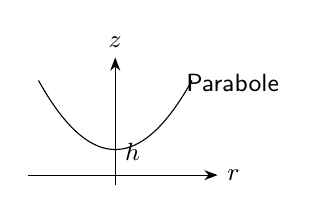
\begin{tikzpicture}[scale=.65]
\draw[->] (-1.7,0)--(2,0) node[right]{$r$};\draw[->] (0,-.2)--(0,2.3) node[above]{$z$};\draw[domain=-1.5:1.5,smooth,variable=\x] plot ({\x},{.5+.6*\x*\x});\node[right] at (0,.45){$h$};\node[right] at (1.2,1.8){Parabole};
\end{tikzpicture}\end{minipage}
\titr{Complément : fluide non compressible}
$\mu\ne\cste$ : cf. TD F1, ultracentrifugation.
\titr{Complément : poussée d'Archimède}
\begin{minipage}{.35\linewidth}\centering\cuve{3}\end{minipage}\hfill\begin{minipage}{.62\linewidth}
Pour trouver $h$, on utilise la conservation de la matière. Dans le cas d'un fluide incompressible, on utilise la conservation du volume.
\end{minipage}
\[
 h_0\pi R^2=h\pi R^2+\iint_{\substack{r:0\to R\\\theta:0\to2\pi}}
 \underbrace{r\,\dd r\,\dd\theta}_{\substack{=\dd^2S\text{ pour une surface}\\\text{horizontale en coordonnées polaires}}}
 \left(\frac{\omega^2r^2}{2g}\right).
\]
\[h_0\pi R^2=h\pi R^2+2\pi\int_0^R\frac{\omega^2}{2g}r^3\,\dd r
=h\pi R^2+\frac{\pi\omega^2R^4}{4g}.\]
\end{document}